\section{Predictive Controls and Their Full Interpretation}
\label{app:predictive-controls}
\Cref{tab:main-findings} preserves the three original-bank predictive findings; \cref{tab:identification-summary} retains the detailed endpoint-by-endpoint comparison. Compare losses within each endpoint: Study~1's $D$, compact-coordinate prediction and context-difference transport use different denominators and sampling contracts.

% Existing reviewed values only; see main_findings.source.json.
\begin{table*}[t]
\caption{Three original-bank findings motivating the completed follow-up. The later authored-context protocol reverses the D4 transport contrast while also changing wording, validation selection and action weights. Smaller losses are better. Category and budget results use the Study~2 compact-comparison training-coordinate-energy denominator; context differences use a separate difference-energy denominator. Each group contains 24 fixed model/readout cells. Compact prediction averages actions equally; the original-bank transport comparison pools changed-state pairs and changes both fitting targets and regularization selection between arms. Targets and changed-state masks are registration-specific, so cross-registration means compare distinct tasks. Full recovery, generator and restricted-registration contrasts remain in \cref{tab:identification-summary}; \cref{sec:setup} defines the descriptive statistical scope.}
\label{tab:main-findings}
\centering\small
\setlength{\tabcolsep}{4pt}
\renewcommand{\arraystretch}{1.10}
\begin{tabular}{@{}p{.23\textwidth}p{.39\textwidth}p{.34\textwidth}@{}}
\toprule
Finding & Existing evidence ($C_7$ / $D_4$) & Interpretation \\
\midrule
Recovery admits competitive alternatives & Centroid: 0.012013 / 0.063821.\newline Ridge: 0.014897 / 0.041919.\newline Centroid lower in 9/24 / 2/24 cells. & Category information improves the $C_7$ mean, not most cells. The control receives labels and the action table; a coherent registration is also competitive. \\
\addlinespace[3pt]
Rankings depend on storage & Nystr\"om first improves both group means at $2\times$; RFF at $4\times$ nominal storage (\cref{fig:budget-frontier}). & All budgets are retained. Parameter storage does not match statistical capacity or runtime memory. \\
\addlinespace[3pt]
An original-bank fitting/selection comparison & Coordinate fit: 0.047137 / 0.132304.\newline Difference fit: 0.034260 / 0.116386.\newline Coherent fit: 0.034465 / 0.117165. & The later authored-context protocol reverses the D4 contrast (Table~\ref{tab:followup-context}); it does not isolate wording alone. Close cross-registration means do not establish semantic preference. \\
\bottomrule
\end{tabular}
\end{table*}


\subsection{Prediction and consistency: two properties, coupled evidence}
Independent ridge attains $\Eeq=0.04830/0.05200$ for $C_7/D_4$, while joint errors are $0.04934/0.05286$. Joint fitting reduces the mean data-space relation defect $\Erel$ by $0.01699/0.00728$ at a small direct-fit cost. The maps support approximate predictive action structure without group-law penalties in the independent objective. However, \cref{prop:propagation} explains why this is not automatically an additional semantic discovery beyond accurate prediction. These diagnostics do not establish a comparison matched in prediction error and operator norm.

Generator-only fits predict five excluded nonidentity elements in each group. Their errors are $0.074443$ for $C_7$ and $0.056558$ for $D_4$. Directly fitted elements yield errors of $0.051124$ and $0.050032$, respectively. The mean correct-minus-length-matched-wrong-word contrast in $D_4$ generator-composed prediction error $E_{\mathrm{gen,eq}}$ is $-1.097329$, with both words scored against the same prescribed targets. This is meaningful transfer in the operator index; the component states and vocabulary were seen in training. Full structural and generator tables, their recorded intervals and depth curves are retained in \cref{app:results}.

\subsection{Invalid registration differs from a coherent alternative}
In the group-label registration control, true-registration homomorphism scores lie below the non-automorphic reference's 2.5\% quantile in all 120 model--depth--split cells per group and metric ($6\times4\times5$), not 120 candidate state-action images. Its restricted ensemble excludes the observed registration; no calibrated semantic-null inference is claimed. The training-correspondence controls refit ridge on corrupted training pairs; errors increase against unchanged true held-out targets. Ordinary predictors can degrade similarly, so this establishes sensitivity to supervision rather than semantic specificity.

Study~2 instead consistently supervises an alternative action induced by swapping two state labels. It preserves group laws and fixed-point counts. All-element ridge errors for the specified/coherent correspondence are $0.014897/0.017503$ in $C_7$ and $0.041919/0.041871$ in $D_4$. Each correspondence uses the same underlying source bank and abstract action labels, but its own targets and changed-state evaluation mask. In $D_4$, conjugacy preserves fixed-point counts while potentially changing their identities, so the scored source/action rows need not coincide. This compares the predictability of two registered tasks, rather than two predictors on identical target rows. The single conjugate alternative remains competitive descriptively despite the invalid-registration separation; it does not characterize all semantic alternatives or nonisomorphic representations.

The exhaustive comparison in \cref{app:pending-protocols} uses spectral budgets on complete banks under their own second-moment metrics, rather than these fitted prediction scores. Its rankings do not order the unknown exact-action risks. Within-template centering changes the budget rankings, and the original corner-image lead disappears even with the original whitening retained (\cref{app:template-centering-sensitivity}). Predictive competitiveness and metric-dependent registration preference concern different endpoints.

\subsection{Predictor rankings change with information and storage}
The nonlinear and category-based predictors below are predictive comparators; their inclusion does not establish exact nonlinear group actions. The common-loss risk comparison in \cref{eq:class-loss-main} separates independent linear maps, independent orthogonal maps, and exact orthogonal actions.

Rank-matched embedding fits are near exact at $q=6$ for weekdays and $q=3$ for corners; internal errors are higher in the two-model lexical panel. Here matching concerns training projected ranks, supported by the audited input spectra and recorded PCA construction at both readouts. The historical projected arrays are unavailable for direct remeasurement (\cref{app:dimension-rank-audit}). \Cref{prop:finite} explains why affinely independent lexical state vectors, after retaining their full centered span, can support exact linear permutation actions without group-specific semantic learning. Matching training rank does not match retained information: the leading 6 or 3 directions of the internal training inputs account for substantially less than their full variance, whereas they span the centered lexical inputs. This comparison does not order all intrinsic structure at the two locations.

In Study~2 at $q=16$, the decoded-centroid predictor improves the $C_7$ mean but wins only 9/24 cells; it is worse on the $D_4$ mean and wins in 2/24. It receives training state labels and the exact action table, beyond source-coordinate/action access. This is an explanatory control with an information advantage. \Cref{tab:main-findings} uses the compact extension's equal-action aggregate; the earlier characterization uses a pooled changed-pair aggregate. For D4, differing fixed-point counts make those weights unequal, so the two recorded means need not agree (\cref{app:aggregation-contract}).

The compact nonlinear comparison fits RFF and Nystr\"om residual predictors using all construction pairs for each fitted nonidentity action, including its fixed points. Neither improves the group mean at the identity-pruned linear storage budget; Nystr\"om does at $2\times$ storage and RFF at $4\times$ in both groups. \Cref{fig:budget-frontier} shows all five declared nominal budgets; exact means and unit-budget comparisons remain in \cref{tab:reproduction-budgets,tab:reproduction-compact}. Storage includes predictor features, normalizers, coefficients and biases, but excludes shared PCA, model weights and runtime memory. The ranking is estimator- and budget-dependent, not universal linear superiority or total-compute efficiency. These nonlinear predictors are shared across contexts, but their prediction scores do not establish invertibility or group laws. Budgets were not selected retrospectively as deployment operating points.

\subsection{A transport advantage within the original construction}
Fitting context differences directly yields losses $0.03426/0.11639$ for $C_7/D_4$, versus $0.04714/0.13230$ for applying coordinate-fitted operators to those differences. The coherent action gives $0.03446/0.11717$ under the same direct fitting procedure and registration-specific scoring just described. The earlier characterization compared difference-fitted maps with scalar retention. This original-bank extension instead compares difference- and coordinate-fitted maps, changing both the training target and regularization selection. Its improvement describes the specified procedures rather than an isolated effect of the fitting objective. Close means for distinct registered tasks establish neither semantic preference nor equivalence. Matched-state context differences cancel state means but retain context main effects, so this endpoint does not isolate state--context interactions. A fitted difference predictor also need not define a group action on the original coordinates. On jointly new $S_3$ contexts/entities, direct transport loss is $0.016290$ versus identity $0.016444$, a small absolute improvement below the inherited $0.01$ practical margin. Complete normalization and information conditions are in \cref{app:characterization,app:reproduction}. On the new authored bank, difference fitting retains a lower loss than coordinate fitting in C7 and has a higher loss in D4 (\cref{tab:followup-context}). Identity has the lowest C7 mean. The old and new studies differ jointly in wording, validation selection and, for D4, state--action weighting (\cref{app:pending-protocols}).

\paragraph{Behavioral scope.}
The activation-edit comparisons supply limited behavioral evidence: the $C_7$ target-logit contrast against the unpatched forward is 1.129, but the mean effect is smaller than that of the source-conditioned additive control. The historical label identity denotes that unpatched baseline. Correct $D_4$ ordering has lower final-logit distance than the matched wrong ordering. These are token/logit outcomes, not a certified native algorithm. The additive control uses full-hidden displacements and source identity. The learned map changes the PCA component of the span mean while retaining that mean's orthogonal residual. The hook then writes the same full-hidden replacement to every selected token. For multi-token spans it removes token-specific deviations, including components outside PCA, so the token-level intervention is not restricted to the PCA subspace. No matched mean-overwrite zero-delta sham was recorded. The separate native program branch failed clean competence and its confirmation remains blocked. Full endpoints and limits, including the unchanged failure records, are in \cref{app:behavior,app:reproduction}.


\begin{figure}[H]
\centering
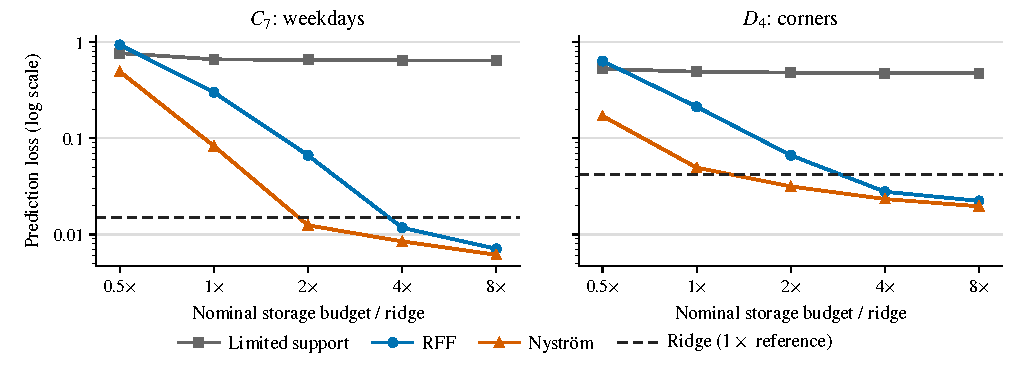
\includegraphics[width=\textwidth]{figures/budget_frontier.pdf}
\caption{\textbf{Predictor rankings change with storage.} Recorded direct-prediction means for all nonidentity actions on changed states under the specified semantic registration, over 24 fixed model/readout cells per domain. Losses use the Study~2 compact-comparison training-coordinate-energy denominator; lower is better. The horizontal axis is the nominal incremental parameter-storage budget relative to identity-pruned ridge, not runtime memory or statistical capacity. All five declared budgets and all three budgeted predictor families are shown. Nystr\"om first improves the group mean over ridge at $2\times$, and RFF at $4\times$, in both groups. Lines connect recorded aggregates on logarithmic axes; they are not fitted scaling laws or confidence bands. This direct-prediction endpoint is distinct from generator-only composition.}
\label{fig:budget-frontier}
\end{figure}

\subsection{Detailed interpretation questions}
\label{app:detailed-reading-protocol}
The findings motivate four complementary questions, conditional on states, contexts, coordinates, estimator and outcome. They organize interpretation rather than define a calibrated certification test or four statistically independent sources of evidence.

\paragraph{1. Predictive recovery.}
State what was held out: contexts, action elements, state identities or domains. Disclose comparator supervision and storage. Our generator result demonstrates why the distinction matters: transfer to an excluded action element can still use a completely familiar state vocabulary.

\paragraph{2. Action consistency.}
Specify the group-law residual, its metric and whether fitting encouraged it. The propagation identity relates consistency to prediction errors and operator norms. Additional semantic interpretation of these fitted diagnostics requires accounting for those quantities; separate objectives alone do not establish independent evidence. The same-bank class-risk comparison asks a different question by computing the independent linear and orthogonal optima and bounding the best exact-action risk under one common loss.

\paragraph{3. Preferential semantic alignment.}
Compare coherent alternatives as well as invalid registrations, making information, capacity, scoring rows, target definitions and predictive difficulty explicit. Our comparisons show why these controls answer different questions. Preference over selected alternatives would narrow the interpretation, rather than identify a unique semantic mechanism.

\paragraph{4. Native causal use.}
For a claim about successful native computation, establish clean-task competence and intervention fidelity, then distinguish sufficiency from necessity for the proposed mechanism. These activation edits illustrate the gap between moving an output score and identifying the computation used by the unedited model.

For a new application, specify the intended claim and competing explanation before choosing a diagnostic. The useful outcome is the interpretation changed by the comparison, including unfavorable results, rather than the number of positive scores obtained.

